\documentclass[tikz,border=5mm]{standalone}
\usepackage{pgfplots}
\usepackage{amsmath}
\pgfplotsset{compat=1.18}

\definecolor{parabolablue}{RGB}{0, 0, 128}
\definecolor{shortred}{RGB}{214, 24, 66}
\definecolor{tangentgreen}{RGB}{0, 100, 0}

\begin{document}
	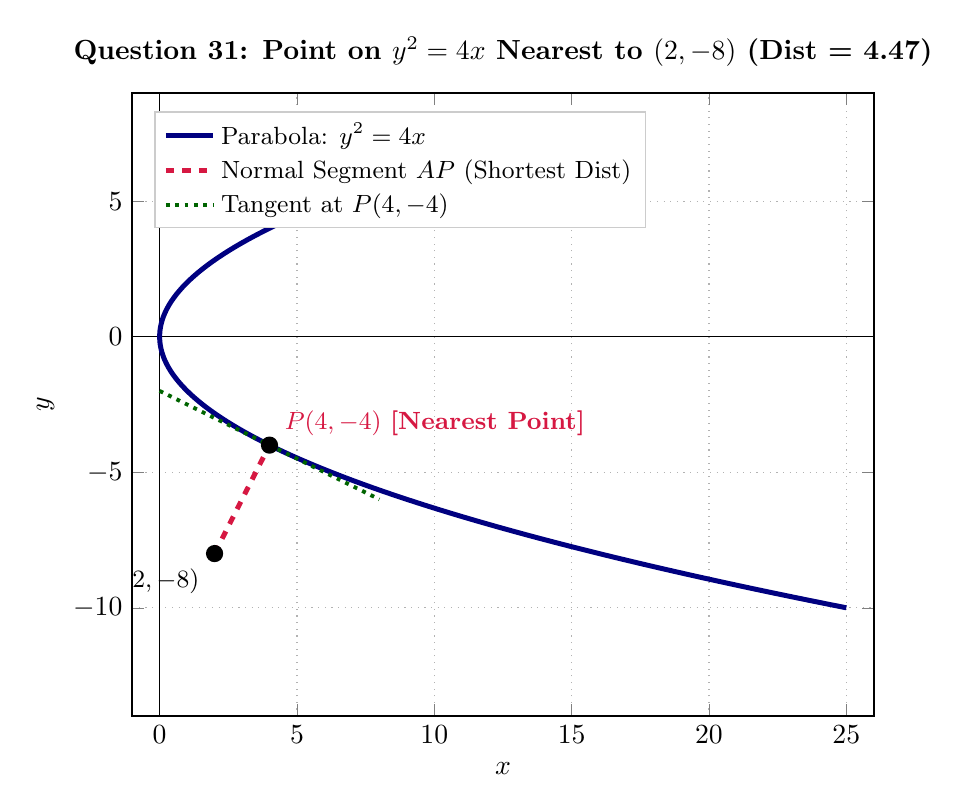
\begin{tikzpicture}
		\begin{axis}[
			width=11cm, height=9.5cm,
			title={\textbf{Question 31: Point on $y^2 = 4x$ Nearest to $(2, -8)$ (Dist = 4.47)}},
			xlabel={$x$}, ylabel={$y$},
			xmin=-1, xmax=26,
			ymin=-14, ymax=9,
			xtick={0, 5, 10, 15, 20, 25},
			ytick={-10, -5, 0, 5},
			grid=both,
			grid style={dotted, gray!60},
			axis line style={black, thick},
			legend cell align={left},
			legend style={at={(0.03,0.97)}, anchor=north west, font=\small, draw=gray!40}
			]
			% Origin axis lines
			\draw[black, thin] (axis cs:0,-14) -- (axis cs:0,9);
			\draw[black, thin] (axis cs:-1,0) -- (axis cs:26,0);
			
			% Parabola y^2 = 4x -> x = y^2 / 4
			\addplot[parabolablue, line width=1.8pt, domain=-10:6, samples=120] ({x^2/4}, {x});
			\addlegendentry{Parabola: $y^2 = 4x$}
			
			% Normal Segment AP: (2, -8) to (4, -4)
			\addplot[shortred, dashed, line width=1.8pt] coordinates {(2, -8) (4, -4)};
			\addlegendentry{Normal Segment $AP$ (Shortest Dist)}
			
			% Tangent line at P(4, -4): y = -0.5x - 2
			\addplot[tangentgreen, dotted, line width=1.4pt, domain=0:8] {-0.5*x - 2};
			\addlegendentry{Tangent at $P(4, -4)$}
			
			% Points
			\node[circle, fill=black, inner sep=2.2pt] at (axis cs:2,-8) {};
			\node[below left=2pt, font=\small] at (axis cs:2,-8) {$A(2, -8)$};
			
			\node[circle, fill=black, inner sep=2.2pt] at (axis cs:4,-4) {};
			\node[anchor=south west, font=\small, text=shortred, xshift=2pt] at (axis cs:4,-4) {$P(4, -4)$ \textbf{[Nearest Point]}};
		\end{axis}
	\end{tikzpicture}
\end{document}